\section{Ling Αθροιστές}
Στα προηγούμενα κεφάλαια παρουσιάστηκαν διάφοροι δυαδικοί αθροιστές , 
ανάμεσα σε αυτούς και ο αθροιστής πρόβλεψης κρατουμένου. Επειτα γνωστοποιήθηκαν 
διάφοροι τρόποι υπολογισμού των κρατουμένων για την υλοποίηση του CLA. Όπως, λοιπον,
έχει αποδειχθεί, οι δομές CLA είναι ιδανικές για την ελάττωση της καθυστέρησης υπολογισμού
του αποτελέσματος. Παρ' όλ' αυτά στο παρόν κεφάλαιο θα παρουσιαστεί μια βελτίωση που προτάθηκε 
από τον Ling \cite{ling}.



\subsection{Βασική Θεωρία}

Ξεκινώντας από την παρακάτω ισότητα 
\begin{equation}
    g_i = g_i*p_i
\end{equation}
\\
η οποία πηγάζει από 
\begin{equation*}
    a_i * b_i = a_i * b_i * (a_i + b_i)
\end{equation*}

Η βασική βελτιστοποίηση που επέφερε η θεωρία του Ling είναι η παρακάτω τροποποίηση 
της συνάρτησης υπολογισμού του σήματος Group Carry Generate του συνόλου $i$ εως $j$ με $i > j$
\begin{equation}
\begin{split}
    G_{i:j} &= g_i + p_ig_{i-1} + p_ip_{i-1}g_{i-2} + ... + p_ip_{i-1}p_{i-1}...p_{j+1}p_j\\
            &= p_ig_i + p_ig_{i-1} + p_ip_{i-1}g_{i-2} + ... + p_ip_{i-1}p_{i-1}...p_{j+1}p_j\\
            &= p_i \bigg[ g_i + g_{i-1} + p_{i-1}g_{i-2} + ... + p_{i-1}p_{i-1}...p_{j+1}p_j \bigg]
\end{split}
\end{equation}
Η τροποποίηση της συνάρτησης $G$ δημιουργεί έναν όρο μέσα στις αγκύλες ο οποίος
ονομάζεται $H$ κατά Ling και έχει τον παρακάτω ορισμό 
\begin{equation}
    H_{i:j} = g_i + G_{i-1:j}
\end{equation}
Επιπλέον για την ανάκτηση του σήματος $G$, δηλαδή του κρατούμενου που παράγει ένα σύνολο, 
που είναι και ο αρχικός σκοπός των CLA αθροιστών γίνεται με την παρακάτω συνάρτηση :
\begin{equation}
    G_{i:j} = p_i * H_{i:j}
\end{equation}
Σημαντικό, επίσης, αυτής της παραγοντοποίησης αυτής είναι πως υποστηρίζεται ο τελεστής $\circledast$
και η αναγωγή της σε πρόβλημα προθέματος. Έχοντας το σύνολο $i$ εως $j$ με $i>k>j$ αποδεικνύεται πως
\begin{equation}
\begin{split}
    G_{i:j} &= G_{i:k} + P_{i:k}*G_{k-1:j}\\
    p_i * H_{i:j}  &= p_i * H_{i:k} + P_{i:k}*\big( p_{k-1}*H_{k-1:j}\big)\\
            &= p_i \big[  H_{i:k} + P_{i-1:k-1}*H_{k-1:j}    \big] \\
    H_{i:j}  &= H_{i:k} + P_{i-1:k-1}*H_{k-1:j}
\end{split}
\end{equation}
\\
Ακολουθεί ένα απλό παράδειγμα για καλύτερη εμπέδωση αλλά και επαλήθευση 
\begin{equation*}
\begin{split}
    H_{7:2} &= H_{7:5} + P_{6:4}*H_{4:2} \\
    H_{7:5} &= g_7 + g_6 + p_6g_5 \\
    H_{4:2} &= g_4 + g_3 + p_3g_2 \\
    P_{6:4} &= p_6p_5p_4\\
    H_{7:2} &= g_7 + g_6 + p_6g_5 + p_6p_5p_4*\big(g_4 + g_3 + p_3g_2 \big)\\
    H_{7:2} &= g_7 + g_6 + p_6g_5 + p_6p_5g_4 + p_6p_5p_4g_3 + p_6p_5p_4p_3g_2
\end{split}
\end{equation*}
Εφόσον στην παραγοντοποίηση που σύστησε ο Ling έχουν κληρονομηθεί όλα τα προνόμια 
των προθεματικών αθροιστών μένει η έκφραση του αποτελέσματος συναρτήσει του σήματος $H$.
Ως γνωστόν, κάθε ένα δυαδικό ψηφίο του αθροίσματος με την τεχνική πρόβλεψης κρατουμένου 
υπολογιζόταν με την συνάρτηση $sum_i = G_{i-1:0} \oplus x_i $ οπου $x_i = a_i \oplus b_i$.
Τελικά, το άθροισμα με την παραγοντοποίηση του Ling υπολογίζεται με :
\begin{equation}
\label{eq:ling_sum_1}
\equationame{άθροισμα κατά Ling}
\begin{split}
    sum_i &= G_{i-1:0} \oplus x_i \\
          &= (p_{i-1} * H_{i-1:0}) \oplus x_i
\end{split}
\end{equation}












\subsection{Πλεονεκτήματα της Ling παραγοντοποίησης}
Ένας αθροιστής Ling βελτιστοποιεί την επίδοση του CLA μειώνοντας κατά ένα το πλήθος 
εισόδων των λογικών πυλών (fan-in). Όμως αφαιρώντας από κάθε όρο του Group Generate 
σήματος ενα propagate έχει ως αποτέλεσμα να αυξάνεται η πολυπλοκότητα του τελευταίου 
σταδίου όπου υπολογίζεται το άθροισμα (εξίσωση [\ref{eq:ling_sum_1}]). 
Παρατηρείται στην εξίσωση \ref{eq:ling_sum_1} πως πρέπει να υπολογιστεί το $H$ 
στην συνέχεια να πραγματοποιηθεί η λογική του πράξη AND με το σήμα $p_i$ και τέλος
η έξοδος της πύλης AND να οδηγήσει την είσοδο της πύλης XOR σε συνδυασμό με το
σήμα $x_i$ ( Εικόνα \ref{fig:Ling_sum_1} ).

\begin{figure}[H]
    \centering
    \begin{subfigure}{.4\textwidth}
        \centering
        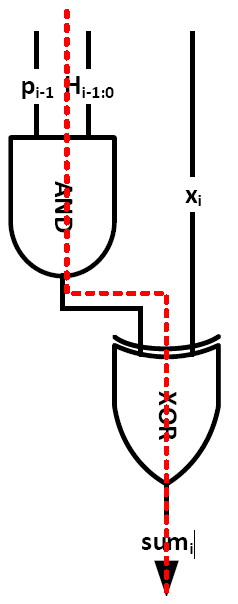
\includegraphics[scale=0.7]{Ling_sum_1.png}
        \caption{Απλή προσέγγιση}
        \label{fig:Ling_sum_1}
    \end{subfigure}
    \begin{subfigure}{.4\textwidth}
        \centering
        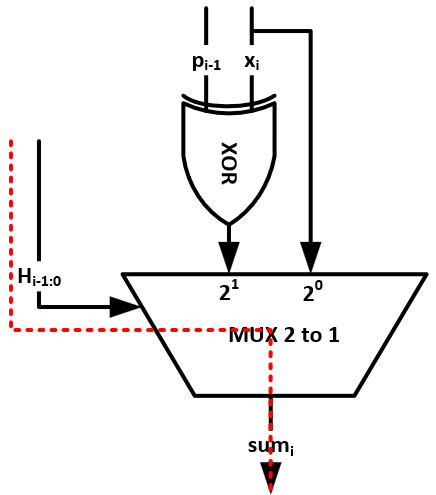
\includegraphics[scale=0.7]{Ling_sum_2.png}
        \caption{Εναλλακτική προσέγγιση με πολυπλέκτη}
        \label{fig:Ling_sum_2}
    \end{subfigure}
    \caption{Λογική υπολογισμού του αθροίσματος κατά Ling}
    \label{fig:Ling_sum}
\end{figure}


% \\\\
% \textcolor{red}{[Figure with logic diagram of whats described above}
% \\\\
Η εξίσωση \ref{eq:ling_sum_1} αυτή μπορεί να εκφραστεί με μεγαλύτερη πολυπλοκότητα 
αλλά ταυτόχρονα μειώνοντας τον συνολικό χρόνο υπολογισμού του αθροίσματος.
\begin{equation}
\label{eq:ling_sum_2}
\equationame{άθροισμα κατά Ling (2)}
    sum_i = H_{i-1:0} ? \big(p_{i-1} \oplus x_i\big) : x_i
\end{equation}
% \\\\
% \textcolor{red}{[Figure with logic diagram of whats described above}
% \\\\
Στην εναλλακτική τροποποίηση που εκφράζεται στην εξίσωση \ref{eq:ling_sum_2} και 
απεικονίζεται στην εικόνα \ref{fig:Ling_sum_2} με πρώτη ματιά φαίνεται να είναι 
υπάρχει αρνητική απόδοση σε σχέση με την αρχική και πιο απλή υλοποίηση.
Στην πραγματικότητα όμως η απόδοση αφορά την καθυστέρησή και όχι το εμβαδόν. Το σήμα
$Η$ είναι αυτό που υπολογίζεται τελευταίο χρονικά και στην πρώτη αρχιτεκτονική
είναι στο κρίσιμο μονοπάτι\footnote{Κρίσιμο μονοπάτι (critical path) Το μονοπάτι με αρχί την είσοδο και τέλος την έξοδο του κυκλώματος που έχει την μεγαλύτερη καθυστέρηση}. Αντίθετα στην δεύτερη υλοποίηση η λογική πύλη XOR 
έχει τελική τιμή στην έξοδο της πριν οριστικοποιηθεί η τιμή του σήματος H, παράλληλα 
με τον υπολογισμό της. 
\\\\
 \textcolor{red}{[Ίσως να ήταν ενδιαφέρον να φτιαχτούν αυτά τα δύο modules και να μετρηθεί 
 το εμβαδόν και το delay τους στο Design Compiler]}
\\

%------------------------------------------------
 Παρατηρούμε πως η μέθοδος του Ling μειώνει την πολυπλοκότητα μόνο στο πρώτο επίπεδο 
 του αθροιστή
 
 
 
 
 
 
 \subsection{Αραίωση σε Ling Αρχιτεκτονικές}
Sparsness-2
\begin{equation*}
    \begin{split}
        sum_i &= x_i \oplus G_{i-1:0}\\
        sum_i &= x_i \oplus p_{i-1}*H_{i-1:0}\\
        sum_i &= H_{i-1:0} ? x_i \oplus p_{i-1} : x_i\\
        sum_{i+1} &= x_{i+1} \oplus G_{i:0}\\
        sum_{i+1} &= x_{i+1} \oplus (g_i + p_i*G_{i-1:0})\\
        sum_{i+1} &= x_{i+1} \oplus (g_i + p_i*p_{i-1}*H_{i-1:0})\\
        sum_{i+1} &= H_{i-1:0} ? x_{i+1} \oplus (g_i + p_i*p_{i-1}) : x_{i+1} \oplus g_i
    \end{split} 
\end{equation*}
Sparsness-4
\begin{equation*}
    \begin{split}
        sum_i =& x_i \oplus G_{i-1:0}\\
        =& x_i \oplus p_{i-1}*H_{i-1:0}\\
        =& H_{i-1:0} ? x_i \oplus p_{i-1} : x_i\\
        sum_{i+1} =& x_{i+1} \oplus G_{i:0}\\
        =& x_{i+1} \oplus (g_i + p_i*G_{i-1:0})\\
        =& x_{i+1} \oplus (g_i + p_i*p_{i-1}*H_{i-1:0})\\
        =& H_{i-1:0} ? x_{i+1} \oplus (g_i + p_i*p_{i-1}) : x_{i+1} \oplus g_i\\
        sum_{i+2} =& x_{i+2} \oplus G_{i+1:0}\\
        =& x_{i+2} \oplus (g_{i+1} + p_{i+1}g_i + p_{i+1}p_iG_{i-1:0})\\
        =& x_{i+2} \oplus (g_{i+1} + p_{i+1}g_i + p_{i+1}p_ip_{i-1}*H_{i-1:0})\\
        =& H_{i-1:0} ? x_{i+2} \oplus (g_{i+1} + p_{i+1}g_i + p_{i+1}p_ip_{i-1}) : x_{i+2} \oplus (g_{i+1} + p_{i+1}g_i)\\
        sum_{i+3} =& x_{i+3} \oplus G_{i+2:0}\\
        =& x_{i+3} \oplus (g_{i+2} + p_{i+2}g_{i+1} + p_{i+2}p_{i+1}g_i + p_{i+2}p_{i+1}p_iG_{i-1:0})\\
        =& x_{i+3} \oplus (g_{i+2} + p_{i+2}g_{i+1} + p_{i+2}p_{i+1}g_i + p_{i+2}p_{i+1}p_ip_{i-1}*H_{i-1:0})\\
        =& H_{i-1:0} ? x_{i+3} \oplus (g_{i+2} + p_{i+2}g_{i+1} + p_{i+2}p_{i+1}g_i + p_{i+2}p_{i+1}p_ip_{i-1}) \\&: x_{i+3} \oplus (g_{i+2} + p_{i+2}g_{i+1} + p_{i+2}p_{i+1}g_i)
    \end{split} 
\end{equation*}

 
 